\documentclass[a4paper]{report}
\input{header.tex}
\author{Haolin Li}
\title{Nonlinear Optimization Notes}

\thispagestyle{empty}
\addbibresource{ref.bib}

\usepackage{adjustbox}
\usepackage{centernot}

\begin{document}

\maketitle

\begin{abstract}
	This course explores unconstrained optimization problems. We begin with conditions for optimality and basic ingredients, like results from convexity. Then go through algorithms that have great impact over this field of study together with analysis on their convergence behavior under certain conditions.
\end{abstract}

\newpage

\tableofcontents

\chapter{Introduction and Recap}

In this chapter, we will go through ideas that inspired the development of this field of study, together with math required for this class and  some basic results from convexity analysis. The kind of problem we are trying to answer has the form:

\begin{mini}
    {x \in \mathbb{R}^d}
    {f(x)} \\
    {}
\end{mini}

Often in machine learning, what we care more about is not the value itself, but the minimizer associated with. Because the objective $f(x)$ serves as a loss function, and what we want is the parameters. As a result, we sometimes slightly change the formation into:
\begin{argmini}
    {x \in \mathbb{R}^d}
    {f(x)} \\
    {}
\end{argmini}

\section{Calculus Review}
\indent Given a function $f(x) \in \mathbb{R}^d \rightarrow \mathbb{R}$, if it's smooth, then we can define its gradient as 
\begin{equation*}
    \nabla f(x) = 
    \begin{pmatrix}
        \frac{\partial f}{\partial x_1} \\
        \vdots \\
        \frac{\partial f}{\partial x_n}
    \end{pmatrix}
\end{equation*}
The gradient at point $x$ is the direction of steepest growth. It originates from the attempt to find a local approximation for any smooth function with an affine function. Specifically, the affine approximation is:
\begin{equation*}
    \tilde{x} \mapsto f(x) + \nabla f^T(x)(\tilde{x} - x)
\end{equation*}
\begin{note}
    Even if $f(x)$ has partial derivatives for all of the coordinates, the gradient might not exists. Take $f(x) = \sqrt{x_1^2 + x_2^2}$ as an example. 
\end{note}

A natural idea is can we find a better approximation with a quadratic? If $f(x)$ is twice differentiable, the Hessian $\nabla^2f(x): \mathbb{R}^d \rightarrow \mathbb{R}^d$ helps our approximation with the following quadratic form:
\begin{equation*}
    \tilde{x} \mapsto f(x) + \nabla f^T(x)(\tilde{x}-x) + (\tilde{x}-x)^T\nabla^2 f(x)(\tilde{x}-x)
\end{equation*}
It's not hard to see that these are just special cases of the Taylor Series for high dimensional functions. But in optimization problems we mostly/only care about the first and second derivetives because of the optimality conditions that we will be talking about later on. No matter affine or quadratic, they are all approximations, so exactly how much deviation do they have is important. Before that, we introduce a tool we will find handy in the future.

\begin{definition}
    Given $f:\mathbb{R}^d \rightarrow \mathbb{R}$, for any $x, s \in \mathbb{R}^d$ fixed, we define the "slice" of $f(x)$ in direction $s$ as:
    \begin{equation*}
        \varphi(t) = f(x + ts)
    \end{equation*}
\end{definition}

\begin{lemma}
    Let $f:\mathbb{R}^d \rightarrow \mathbb{R}$, then $\forall x,s \in \mathbb{R}^d$, the following two statements hold:
    \begin{enumerate}
        \item If $f(x)$ is smooth, so is $\varphi(t)$ with $\varphi'(t) = s^T \nabla f(x+ts)$.
        \item If $f(x)$ is twice differentiable, so is $\varphi(t)$ with $\varphi''(t) = s^T \nabla^2 f(x) s$
    \end{enumerate}
\end{lemma}

It's not hard to see how the differentiability is passed down to $\varphi(t)$. With this lemma, we can upper bound the approximation error in any direction with the following two theorems.

\begin{theorem}[Taylor Expansion First-Order Approximation]
    Let $f(x)$ have L-Lipschitz continuous $\nabla f(x)$. Then for any $x, s \in \mathbb{R}^d$, we have
    \begin{equation}
        | f(x+ts) - (f(x) + t\nabla f^T(x)s) | \leq \frac{L}{2}t^2\|s\|^2
    \end{equation}
    In addition, if $f(x)$ has a Q-Lipschitz Hessian(operator norm). We have
    \begin{equation}
        |f(x + ts) - (f(x) + t \nabla f^T(x)s + \frac{t^2}{2}s^T \nabla^2 f(x)s)| \leq \frac{Q}{6}t^3\|s\|^3
    \end{equation}
\end{theorem}
This means, if we enforce Lipschitz condition on $f(x)$, which is not very strict in practice, then the approximation error can be upper bounded by the square or the cude of $t\|s\|$. This shouldn't be surprising since it matches the residual of Taylor expansion. 


\section{Optimality Conditions}
In this section, we use the proposed theorem to explain why do we care specifically about the first and second derivatives. Local optimality can be checked by examining the first and second order derivatives.

\begin{theorem}[First-order necessary]~\\
    \indent Suppose $f(x) \in C^1$, then $x*$ is a local minimizer$\Rightarrow \; \nabla f(x*) = 0$
\end{theorem}

\begin{theorem}[First-order sufficient]~\\
    \indent Suppose $f(x) \in C^1$ and is also convex, then $x*$ is a local minimizer $\Leftrightarrow \; \nabla f(x*) = 0$
\end{theorem}

\begin{theorem}[Second-order necessary]~\\
    \indent Suppose $f(x) \in C^2$, then $x*$ is a local minimizer $\Rightarrow \; \nabla^2 f(x*) \succeq 0$ 
\end{theorem}

\begin{theorem}[Second-order necessary]~\\
    \indent Suppose $f(x) \in C^2$, then $x*$ is a local minimizer $\Rightarrow \; \nabla^2 f(x*) \succ 0$
\end{theorem}


\section{Basics of Convexity}
\begin{definition}[Convex Set]
    A set $C \subseteq \mathbb{R}^d$ is convex if given any $x,y \in \mathbb{R}^d$ and $\lambda \in [0,1]$, we have $tx + (1-t)y \in C$.
\end{definition}
\begin{definition}[Epigraph]
    Let $f(x): \mathbb{R}^d \rightarrow \mathbb{R}$, then $epi(f) = \{(x, t) : t \geq f(x)\}$
\end{definition}
\begin{lemma}
    $f(x)$ is convex $\Leftrightarrow$ $epi(f)$ is convex
\end{lemma}

\begin{lemma}[Operations Perserving Convexity]
    Assume $C_1, C_2 \subseteq \mathbb{R}^d$ and $C_3 \subseteq \mathbb{R}^n$ are convex sets.
    \begin{enumerate}
        \item (Scaling) $\mathbb{R}_+ \cdot C_1$
        \item (Minkovski Sum) $C_1 + C_2$
        \item (Intersections) $C_1 \cap C_2$
        \item (Affine image and preimage) Let $\mathcal{A}:\mathbb{R}^d \rightarrow \mathbb{R}^n$ be affine, then $\mathcal{A}(C_1)$ and $\mathcal{A}^{-1}C_3$ are convex.
    \end{enumerate}
\end{lemma}

Now we will check how can we characterize smooth convex functions with the gradient.

\begin{proposition}[First-order Characterization of Smooth Convex Function]
    Suppose $f(x): \mathbb{R}^n \rightarrow \mathbb{R}$ is differentiable, then TFAE
    \begin{enumerate}
        \item $f(x)$ is convex
        \item $\forall x,y \in \mathbb{R}^d$, we have $f(y) \leq f(x) + \langle \nabla f(x), y-x \rangle$
        \item $\forall x,y \in \mathbb{R}^d$, we have $\langle \nabla f(y) - \nabla f(x), x-y \rangle \geq 0$
    \end{enumerate}
\end{proposition}
\chapter{Algorithms}

In this section, we will go through several optimization algorithms and some bounds.

\section{Gradient Descent}
One of the most famous and frequently used optimization algorithms is the gradient descent, which can be formulated as:
\begin{equation}\label{eq:GradientDescentUpdateFormula}
    x_{k+1} \leftarrow x_k - \alpha_k\nabla f(x_k)
\end{equation}
Interestingly, this update formula can be interpreted in the following way:
\begin{equation*}
    x_{k+1} = \arg\min_x \{ f(x_k) + \langle \nabla f(x_k), x-x_k \rangle + \frac{1}{2\alpha_k}\|x-x_k\|^2 \}
\end{equation*}
In fact, if we denote $h(x) = f(x_k) + \langle \nabla f(x_k), x-x_k \rangle + \frac{1}{2\alpha_k}\|x-x_k\|^2$, by checking the first-order necessary condition, we have 
\begin{equation*}
    \nabla h(x) = \nabla f(x_k) + \frac{1}{\alpha_k}(x - x_k)
\end{equation*}
By setting $\nabla h(x) = 0$, we derive $x_{k+1} = x = x_k - \alpha_k\nabla f(x_k)$, which is the same as formula \ref{eq:GradientDescentUpdateFormula}.

\begin{note}
    We can see that $h_k(x)$ is the Taylor expansion of $f(x)$ at $x_k$.
\end{note}

Since we are interested in the minimization and maximization potential of the update algorithm, it's worth to explore how the corresponding value $f(x)$ changes. 
\begin{lemma}[Descent Lemma]\label{lemma:DescentLemma}
    Let $f: \mathbb{R}^d \rightarrow \mathbb{R}$ have L-Lipschitz gradient and $k \geq 0$, we have
    \begin{equation*}
        f(x_{k+1}) \leq f(x_k) - (\alpha_k - \frac{L\alpha_k^2}{2}) \| \nabla f(x_k) \|^2
    \end{equation*}
\end{lemma}
\begin{proof}
    Only need to use the first-order Taylor bound:
    \begin{equation*}
        | f(x_{k+1}) - f(x_k) - \langle \nabla f(x_k), x_{k+1} - x_k \rangle | \leq \frac{L}{2}\|x_{k+1} - x_k\|^2
    \end{equation*}
\end{proof}

To minimize $f(x)$, we want the upper bound in lemma \ref{lemma:DescentLemma} to be as small as possible, meaning that we need to maximize $\alpha_k - \frac{L\alpha_k^2}{2}$. By solving this simple quadratic, we derive the ideal step size $\alpha_k = \frac{1}{L}$. However, this can be quite impractical since even if it's not a strong assumption to take functions we see in rea life over a fintie domain as Lipschitz, it can be difficult to determine the Lipschitz constant $L$. If we examine the update formula \ref{eq:GradientDescentUpdateFormula} closely, the only thing that needs external care is the step size $\alpha_k$. As a result, in the following we will discuss how to find a both effectively and pratically way to determine the step size $\alpha_k$.

\subsection{Exact Linesearch}

A straight forward approach is to find the solution of the following optimization problem, which is also referred to as the exact line search:
\begin{equation*}
    \alpha_k = \argmin_{\alpha \in \mathbb{R}}f(x_k - \nabla f(x_k))
\end{equation*}
Yet this can also be impractical because it means we have to solve an optimization problem at each step of update. In replacement to exact linesearch, we introduce the following backtracking linesearch algorithm.

\subsection{Backtracking Linesearch}
The idea of backtracking linesearch is quite simple, we start with a step size large enough, and then shrink it little by little until we observe sufficient descent. This can be formalized with the following two steps:
\begin{enumerate}
    \item Pick $\alpha \in \mathbb{R}_+$ and $\tau \in (0,1)$, decrease step size by $\alpha_n = a\tau^n$.
    \item To measure the descent, we use the so-called Armijo condition.
\end{enumerate}
\begin{definition}[Armijo Condition]
    Pick $\eta \in (0,1)$, declare sufficient descent when $f(x_k - \alpha\nabla f(x_k)) \leq f(x_k) - \eta\alpha\|\nabla f(x_k)\|^2$
\end{definition}

Therefore, we can restate the backtracking algorithm as:
\begin{equation*}
    \alpha_k = \max_n \{ a\tau^n : \text{Armijo condition holds for }\alpha = a\tau^n \}
\end{equation*}
One nice thing about Armijo's condition is that it clarifies the vague term "sufficient decsent". The right hand side of Armijo's condition is affine in $\alpha$, but the descent lemma \ref{lemma:DescentLemma} was in the quadratic of $\alpha$. This implies the existence of an $\alpha$ small enough such that the quadratic bound is lower than the linear bound. To be even clearer, we have the following range for step size $\alpha$.

\begin{lemma}\label{lemma:ArmijoStepSizeBound}
    The Armijo condition holds for 
    \begin{equation*}
        \alpha \in [0, \frac{2(1 - \eta)}{L}]
    \end{equation*}
\end{lemma}
\begin{proof}
    Using the descent lemma, and bound the right hand side with linear upper bound, we have
    \begin{equation*}
        f(x_k - \alpha \nabla f(x_k)) \leq f(x_k) - (\alpha - \frac{L\alpha^2}{2})\|\nabla f(x_k)\|^2 \leq f(x_k) - \eta\alpha\|\nabla f(x_k) \|^2
    \end{equation*}
    This is the same as
    \begin{equation*}
        \eta\alpha \leq \alpha - \frac{L}{2}\alpha^2
    \end{equation*}
\end{proof}

\begin{note}[Consequences of Backtracking Linesearch]
    Firstly, for each search for step size $\alpha$, it needs no more than $\lceil \log_{\frac{1}{\tau}} (\frac{\alpha L}{2(1-\eta)}) \rceil $ steps to terminate. This bound is derived by asking $\alpha \tau^n \leq $ the bound in \ref{lemma:ArmijoStepSizeBound}. Secondly, we have $\alpha_k \geq \min\{ a, \frac{2\tau(1 - \eta)}{L} \}$ because we either find the sufficient descent at the first step, or find it no smaller than $\tau$ times the upper bound in \ref{lemma:ArmijoStepSizeBound}, which is the next iteration of step size. So we can rewrite the Armijo condition as:
    \begin{align}
        f(x_{k+1}) &\leq f(x_k) - \eta \alpha_k\|\nabla f(x_k) \|^2 \\
        &\leq f(x_k) - \eta \min\{ a, \frac{2\tau(1-\eta)}{L} \} \cdot \|\nabla f(x_k) \|^2  \label{eq:ArmijoUpdateSubstituteAlphak}
    \end{align}
    Now in the special case where $a \geq \frac{1}{L}$ and $\eta = \tau = \frac{1}{2}$, we have 
    \begin{align*}
        (\ref{eq:ArmijoUpdateSubstituteAlphak}) &\leq f(x_k) - \frac{1}{2}\min\{\frac{1}{L}, \frac{1}{2L}\} \cdot \|\nabla f(x_k) \|^2 \\
        &\leq f(x_k) - \frac{1}{4L}\| \nabla f(x_k) \|^2
    \end{align*}
    which does not result in a great sacrifice on the tightness of the bound compared with the quadratic in the descent lemma when the step size is small enough or asking $L > 1$.
\end{note}
\chapter{Proximal Method}
In this chapter we will study proximal method which can be seen as a generalization of gradient descent. Before formally introduce the formulation, we will first describe a few examples and how the idea is developed. 

\section{Motivating Problems}
Many problems in real life can be ill-posed due to the lack of information. For example, in solving the linear system

\begin{equation*}
    Ax = b, \quad A \in \mathbb{R}^{n \times p}
\end{equation*}
It can be solved if $A$ is tall and thin, i.e. $n \gg p$. But for most of the time in science, what available is a fat and short one. This means the matrix $A$ is probably not full-rank, which means the solution is not unique. But picking from a space of solution can be subjective sometimes and hard to justify. A natural idea is to add additional restrictions(structure) on top of the existing problem so as to narrow down the parameter space where we are exploring for answers. In this way, we can hope/guarantee the uniqueness of the solution. One way to solve this problem is through adding $L^1$ norm restriction on the parameters $x$, which is also famously known as Lasso regression:
\begin{equation*}
    \min_{x \in \mathbb{R}^d} \|Ax - b\|^2 + \lambda\|x\|_1
\end{equation*}
By adding this restriction, we are favoring smaller parameters in hope for better robustness. 

Another interesting exmaple is the Netflix Recommendation System challenge which can be mathematically formulated as a matrix recovery problem. Given a matrix $X \in \mathbb{R}^{d_1 \times d_2}$ such that
\begin{equation*}
    \mathcal{A}(X) = b
\end{equation*}
where operator $\mathcal{A}$ maps $X \mapsto \mathbb{R}^m$ with $m \ll d_1 \times d_2$. Similarly, in order to preserve the low-rank property, the problem is formulated as:
\begin{equation*}
    \min \|\mathcal{A}(X) - b \|^2_2 + \lambda\|X\|_*
\end{equation*}
where $\| X \|_* = \sum_{i=1}^{\min d_1, d_2}\sigma_i(X)$ refers to the nuclear norm.

\begin{remark}
    The common pattern between the above two examples is that they are all formed in the following way
    \begin{equation*}
        \min_{x} f(x) + h(x)
    \end{equation*}
    where $f(x)$ is smooth/differentiable, and $h(x)$ is convex and has a nice decomposition. 
\end{remark}

This insight leads us into the object we are going to study.

\section{Proximal Operator}
Algorithms are usually inspired by the idea of approximation, just like gradient descent. We proved that the update rule
\begin{equation*}
    x_{k+1} \leftarrow x_k - \alpha_k \nabla f(x_k)
\end{equation*}
is equivalent to solving the following approximation 
\begin{equation*}
    x_{k+1} \leftarrow \argmin \{ f(x_{k}) + \langle \nabla f(x_k), x-x_k \rangle + \frac{1}{2\alpha_k}\|x - x_k\|^2 \}
\end{equation*}

As a result, gradient descent can be viewed as a special case of proximal method where $f(x) = f(x_{k}) + \langle \nabla f(x_k), x-x_k \rangle$ is differentiable, and $h(x) = \frac{1}{2\alpha_k}\|x - x_k\|^2$ is convex. To formulate this, we consider any given closed convex function $\psi : \mathbb{R}^d \rightarrow \mathbb{R}\cup\{+\infty\}$, the proximal operator is defined as
\begin{equation}
    prox_{\alpha \psi}(x) = \argmin_{z \in \mathbb{R}^d} \{ \psi(z) + \frac{1}{2\alpha}\|z - x \|^2 \}
\end{equation}

One thing that needs clarification is that we used $=$ instead of $\in$ in the definition of the proximal operator, this is guaranteed by the fact that $\psi(z) + \frac{1}{2\alpha}\|z - x \|^2$ is a strongly convex function, resulting in a unique minimizer. This gives the following statement.
\begin{lemma}
    The proximal operator is well defined.
\end{lemma}

To solve the general optimization problem, we have the following necessary condition to follow.
\begin{lemma}
    Let $\psi : \mathbb{R}^d \rightarrow \mathbb{R}\cup\{+\infty\}$ be a closed convex function and $f : \mathbb{R}^d \rightarrow \mathbb{R}$ be a smooth function. Let $x^* \in \argmin \psi(x) + f(x)$, then we have
    \begin{equation*}
        - \nabla f(x^*) \in \partial \psi(x^*)
    \end{equation*}
\end{lemma}
\begin{note}
    We can't prove this using subdifferential calculus since it requires both $f(x)$ and $\psi(x)$ to be convex. 
\end{note}

Furthermore, if we ask $f(x)$ to be also convex, for this special case the necessary condition for the proximal operator is described in the following corollary.
\begin{corollary}
    Same configuration as above, with $f(x)$ being convex, then $x^+ = prox_{\alpha\psi}(x) \iff $ 
    \begin{equation*}
        \frac{x - x^+}{\alpha} \in \partial \psi(x^+) 
    \end{equation*}

\end{corollary}
\chapter{Multivariate Normal Model}

Now we have seen a little bit about how Bayesian models work when the sampling random variable maps to a 1-dimensional real number. In this chapter, through the perspective of multivariate normal, we take a tour around the world when 
\begin{equation*}
    X: \mathcal{F} \rightarrow \mathbb{R}^p
\end{equation*}

\section{Semi-Conjugate Prior}
Semi-conjugate modeling requires parameters to be independent to each other, which is easier to begin with. In high dimension cases, each data point/sample looks like this
\begin{equation*}
    Y_i = (Y_{i1}, \ldots, Y_{ip})^T \in \mathbb{R}^p
\end{equation*}

As a semi-conjugate case, the following plot illustrates how will we structure this model. While both $\vec{\theta}, \Sigma$ depends on some latent variables, but they are not implicitely connected in any way. Firstly, we will talk about how we are going to model the prior of $\vec{\theta}$ and leave $\Sigma$'s latent for now. 

\begin{center}
    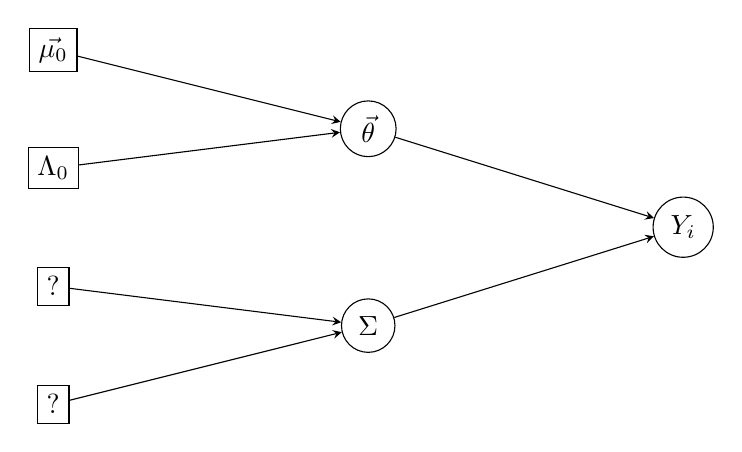
\begin{tikzpicture}[>=stealth, node distance=2cm and 4cm]
    
        % Define nodes in the first column (left)
        \node[draw, rectangle] (A1) at (0,0) {$\vec{\mu_0}$};
        \node[draw, rectangle] (A2) at (0,-1.5) {$\Lambda_0$};
        \node[draw, rectangle] (A3) at (0,-3) { ? };
        \node[draw, rectangle] (A4) at (0,-4.5) { ? };
        
        % Define nodes in the second column (middle)
        \node[draw, circle] (B1) at (4,-1) {$\vec{\theta}$};
        \node[draw, circle] (B2) at (4,-3.5) {$\Sigma$};
        
        % Define node in the third column (right)
        \node[draw, circle] (C1) at (8,-2.25) {$Y_{i}$};
        
        % Draw arrows connecting the first column to the second column
        \draw[->] (A1) -- (B1);
        \draw[->] (A2) -- (B1);
        \draw[->] (A3) -- (B2);
        \draw[->] (A4) -- (B2);
        
        % Draw arrows connecting the second column to the third column
        \draw[->] (B1) -- (C1);
        \draw[->] (B2) -- (C1);
    
    \end{tikzpicture}
\end{center}

\subsection{$\theta$ as Multivariate Normal}
In the 1-dimension case, we modeled $\theta$ as a normal. As a high-dimensional generalization, we choose to model $\vec{\theta}$ as multivariate normal:
\begin{equation*}
    \vec{\theta} \sim MVN(\mu_0, \Lambda_0)
\end{equation*}
If we dive deeper into its pdf, we have the following:
\begin{align*}
    p(\vec{\theta}) &= (2\pi)^{-p/2}|\Lambda_0|^{-1/2} \exp \big( -\frac{1}{2}(\theta - \mu_0)^T \Lambda_0^{-1}(\theta - \mu_0) \big) \\
    &\propto \exp \big( -\frac{1}{2}\theta^T\Lambda_0^{-1}\theta + \frac{1}{2}\theta^T\Lambda_0^{-1}\mu_0 + \frac{1}{2}\mu_0^T\Lambda_0^{-1}\theta - \frac{1}{2}\mu_0^T\Lambda_0^{-1}\mu_0 \big) \\
    &\propto \exp \big( -\frac{1}{2}\theta^T\Lambda_0^{-1}\theta + \theta^T\Lambda_0^{-1}\mu_0 \big) \\ 
    &= \exp \big( -\frac{1}{2}\theta^TA_0\theta + \theta^T b_0 \big)
\end{align*}
where we reparametized $A_0 = \Lambda_0^{-1}$ and $b_0 = A_0\mu_0 = \Lambda_0^{-1}\mu_0$.

As a direct consequence of the reparametrization, we have 
\begin{equation*}
    \vec{\theta} \sim MVN(A_0^{-1}b_0, A_0^{-1})
\end{equation*}

\subsection*{Joint Sampling Model}
Now, assuming we have known $\Sigma$, then our sampling model can be written as 
\begin{align*}
    p(\vec{\theta} | \vec{Y}, \theta, \Sigma) &= \Pi_{i=1}^n (2\pi)^{-p/2} |\Sigma|^{-\frac{1}{2}} \exp \big( -\frac{1}{2}(Y_i - \vec{\theta})^T \Sigma^{-1}(Y_i - \vec{\theta}) \big) \\
    &\propto \exp \big( -\frac{n}{2}\theta^T\Sigma^{-1}\theta + \theta^T\Sigma^{-1}\sum_{i=1}^n Y_i - \frac{1}{2}\sum_{i=1}^n(Y_i^T\Sigma^{-1}Y_i) \big) \\
    &\propto \exp \big( -\frac{1}{2}\theta^TA_1\theta + \theta^Tb_1 \big)
\end{align*}
where we reparametized $A_1 = n\Sigma^{-1}$ and $b_1 = \Sigma^{-1}\sum_{i=1}^nY_i = n\Sigma^{-1}\bar{Y}$

\subsection*{Posterior}
With the sampling and prior, we now formulate the posterior:
\begin{align*}
    p(\vec{\theta} | \vec{Y}, \Sigma) &\propto p(\vec{Y} | \theta, \Sigma) \cdot p(\theta) \\
    &\propto \exp \big( -\frac{1}{2}\theta^TA_1\theta + \theta^Tb_1 \big) \cdot \exp \big( -\frac{1}{2}\theta^TA_0\theta + \theta^Tb_0 \big) \\
    &= \exp \big( -\frac{1}{2}\theta^T(A_0 + A_1)\theta + \theta^T(b_0 + b_1) \big)
\end{align*}
Notice the first line where we used Bayes' rule, we have $p(\theta | \Sigma) = p(\theta)$ because we are modeling the semi-conjugate case. In conclusion, we have obtained the posterior as
\begin{equation*}
    \vec{\theta} | \vec{Y}, \Sigma \sim MVN(A_n^{-1}b_n, A_n^{-1})
\end{equation*}
where $A_n = A_0 + A_1 = \Lambda_0^{-1} + n\Sigma^{-1}$ and $b_n = b_0 + b_1 = \Lambda_0^{-1}\mu_0 + n\Sigma^{-1}\bar{Y}$

\subsection{$\Sigma$ as Inverse-Wishart}
In 1-dimension case, we would model the variance term of normals as $\chi^2_n$. Its high dimensional resemblence is the Wishart distribution. 
\begin{enumerate}
    \item Firstly we sample $z_i \sim MVN(\vec{0}, \Phi_0)$, $i=1, \ldots, \nu_0$
    \item Then we have $\sum_{i=1}^{\nu_0}z_iz_i^T \sim Wishart(\nu_0, \Phi_0)$ 
\end{enumerate}
One thing worth noticing is that we actually can sample PSD fro Wishart, for example the all-zero matrix. However, we are not very concerned with this setback because firstly it's a zero-measure set, secondly we usually tolerates the covariance to be PSD in the sense that there exists colliniarity between variables. Generally speaking, it's sensible to model something that is bound to be PD as Wishart distributed. In conclusion, we have
\begin{equation*}
    \sum_{i=1}^{n}z_iz_i^T \sim Wishart(\nu_0, S_0^{-1})
\end{equation*}
\begin{equation*}
    \Sigma = (\sum_{i=1}^{n}z_iz_i^T)^{-1} \sim InvWishart(\nu_0, S_0^{-1})
\end{equation*}
In other words, we have completed the dependency plot

\begin{center}
    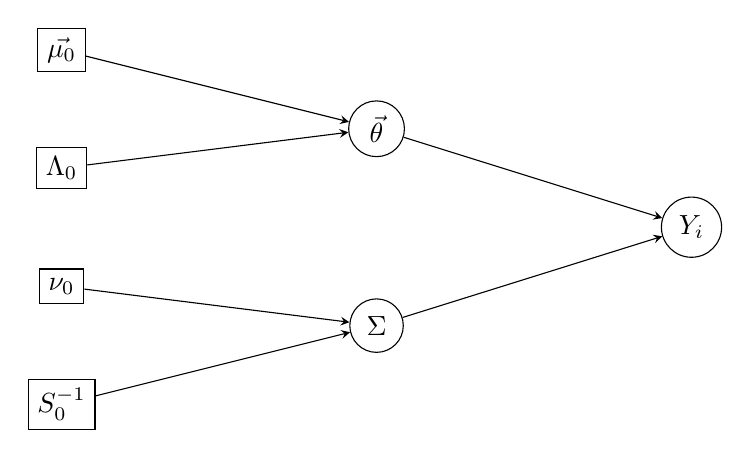
\begin{tikzpicture}[>=stealth, node distance=2cm and 4cm]
    
        % Define nodes in the first column (left)
        \node[draw, rectangle] (A1) at (0,0) {$\vec{\mu_0}$};
        \node[draw, rectangle] (A2) at (0,-1.5) {$\Lambda_0$};
        \node[draw, rectangle] (A3) at (0,-3) { $\nu_0$ };
        \node[draw, rectangle] (A4) at (0,-4.5) { $ S_0^{-1} $ };
        
        % Define nodes in the second column (middle)
        \node[draw, circle] (B1) at (4,-1) {$\vec{\theta}$};
        \node[draw, circle] (B2) at (4,-3.5) {$\Sigma$};
        
        % Define node in the third column (right)
        \node[draw, circle] (C1) at (8,-2.25) {$Y_{i}$};
        
        % Draw arrows connecting the first column to the second column
        \draw[->] (A1) -- (B1);
        \draw[->] (A2) -- (B1);
        \draw[->] (A3) -- (B2);
        \draw[->] (A4) -- (B2);
        
        % Draw arrows connecting the second column to the third column
        \draw[->] (B1) -- (C1);
        \draw[->] (B2) -- (C1);
    
    \end{tikzpicture}
\end{center}


\section{Full-Conjugate Prior}
In the previous section, we have seen how the semi-conjugate case works for modeling MVN-InvWishart prior. Now we take a look at the full-conjugate case. Quite similar to the 1-dimensional case, we add an additional dependency of the mean $\vec{\theta}$ over the covariance matrix $\Sigma$. From base to top, let's dig a little more on the Wishart. 

\begin{center}
    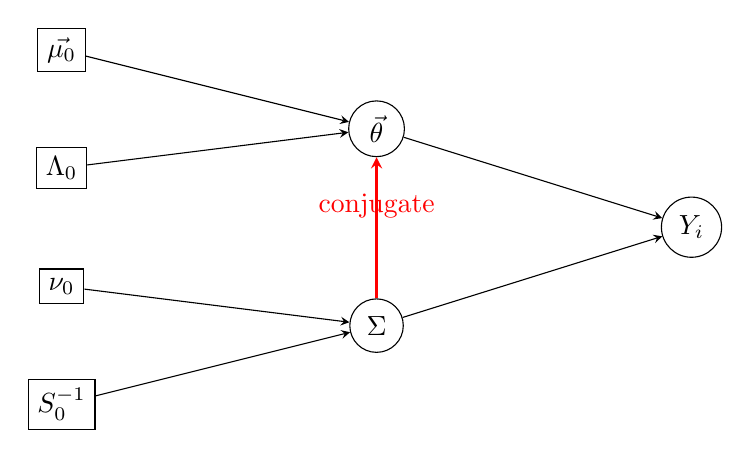
\begin{tikzpicture}[>=stealth, node distance=2cm and 4cm]
    
        % Define nodes in the first column (left)
        \node[draw, rectangle] (A1) at (0,0) {$\vec{\mu_0}$};
        \node[draw, rectangle] (A2) at (0,-1.5) {$\Lambda_0$};
        \node[draw, rectangle] (A3) at (0,-3) { $\nu_0$ };
        \node[draw, rectangle] (A4) at (0,-4.5) { $ S_0^{-1} $ };
        
        % Define nodes in the second column (middle)
        \node[draw, circle] (B1) at (4,-1) {$\vec{\theta}$};
        \node[draw, circle] (B2) at (4,-3.5) {$\Sigma$};
        
        % Define node in the third column (right)
        \node[draw, circle] (C1) at (8,-2.25) {$Y_{i}$};
        
        % Draw arrows connecting the first column to the second column
        \draw[->] (A1) -- (B1);
        \draw[->] (A2) -- (B1);
        \draw[->] (A3) -- (B2);
        \draw[->] (A4) -- (B2);
        
        % Draw arrows connecting the second column to the third column
        \draw[->] (B1) -- (C1);
        \draw[->] (B2) -- (C1);

        \draw[red, thick, ->] (B2) -- (B1) node[midway, above] {conjugate};
    
    \end{tikzpicture}
\end{center}

\subsection{More on Wishart}

\chapter{Hierarchical Models}
Hierarchical model is useful in the sense that it allows between-group information sharing. In contrast, for frequentists, two groups of sample are usually assumed to be drawn from different distributions. A direct result is that the estimation on the average is not a continuum but discrete
\begin{equation*}
    \hat{\theta}_i = 
    \begin{cases}
        \bar{y_i} & \text{if } \mu_1 \neq \mu_2, \\
        \frac{\sum Y_{i1} + \sum Y_{i2}}{n_1 + n_2} & \text{if } \mu_1 = \mu_2.
    \end{cases}
\end{equation*}
An even worse disturbance is that we are only using within-group data, potentially making our estimation less robust. To save the world, the hierarchical Bayesian model is come to the rescue. We start with a simple 2-group case. For simplicity, we will only talk about 1-dimensional distributions.

\section{Two-Group Hierarchy}
Bayesians model the two groups as follow:
\begin{align*}
    Y_{i, 1} &= \mu + \delta + \epsilon_{i, 1} \\
    Y_{i, 2} &= \mu - \delta + \epsilon_{i, 2} \\
    \{\epsilon_{i,j}\} &\sim_{iid} N(0, \sigma^2)
\end{align*}
where the three parameters follows $p(\mu, \delta, \sigma^2) = p(\mu) \times p(\delta) \times p(\sigma^2)$ with
\begin{align*}
    \mu &\sim N(\mu_0, \gamma_0^2) \\
    \delta &\sim N(\delta_0, \tau_0^2) \\
    \sigma^2 \sim& InvGamma(\nu_0/2, \nu_0\sigma_0^2/2)
\end{align*}

\subsection*{Full Conditional}
\begin{equation*}
    \mu | \vec{Y_1}, \vec{Y_2}, \delta, \sigma^2 \sim N(\mu_n, \gamma_n^2)
\end{equation*}
\begin{equation*}
    \delta | \vec{Y_1}, \vec{Y_2}, \mu, \sigma^2 \sim N(\delta_n, \tau_n^2)
\end{equation*}
\begin{equation*}
    \sigma^2 | \vec{Y_1}, \vec{Y_2}, \delta, \mu \sim InvGamma(\nu_n/2, \nu_n\sigma_n^2/2)
\end{equation*}

\subsection*{Model Structure Outline}
\begin{figure}[H]
    \centering
    \includegraphics[width=0.9\textwidth]{~/Documents/Lecture_Notes/2024_FALL_JHU/Bayesian_Statistics/Figures/Hierarchical_Bayesian_Models.png}
\end{figure}

\section{Multigroup Hierarchy}

\subsection*{Prior}
\begin{equation*}
    \sigma^2 \sim InvGamma(\nu_0/2, \nu_0\sigma_0^2/2)
\end{equation*}
\begin{equation*}
    \tau^2 \sim InvGamma(\eta_0/2, \eta_0\tau_0^2/2)
\end{equation*}
\begin{equation*}
    \mu \sim N(\mu_0, \gamma_0^2)
\end{equation*}

\subsection*{Full Conditional Distribution}
We can use the following results to estimate the parameters. 
\begin{equation*}
    \mu | \theta_1, \ldots, \theta_m, \tau^2 \sim N(\frac{m\bar{\theta}/\tau^2 + \mu_0/\gamma_0^2}{m/\tau^2 + 1/\gamma_0^2}, [m/\tau^2 + 1/\gamma_0^2]^{-1})
\end{equation*}
\begin{equation*}
    \tau^2 | \vec{\theta}, \mu \sim InvGamma(\frac{\eta_0 + m}{2}, \frac{\eta_0\tau_0^2 + \sum_{i=1}^{m}(\theta_i - \mu)^2}{2})
\end{equation*}
\begin{equation*}
    \theta_j | \vec{Y_j}, \sigma^2 \sim N(\frac{n_j\bar{y}_j/\sigma^2 + \mu/\tau^2}{n_j/\sigma^2 + 1/\tau^2}, [n_j/\sigma^2 + 1/\tau^2]^{-1})
\end{equation*}
\begin{equation*}
    \sigma^2 | \theta, \vec{Y} \sim InvGamma(\frac{1}{2}\big[\nu_0 + \sum_{j=1}^{m}n_j\big], \frac{1}{2}\big[\nu_0\sigma_0^2 + \sum_{j=1}^{m}\sum_{i=1}^{n_j}(Y_{i,j} - \theta_j)^2\big])
\end{equation*}

\newpage
%─────Appendix────────────────────────────────────────────────────────────────────────────────────────────────────────────────────────────────────────

\newpage
%─────Reference──────────────────────────────────────────────────────────────────────────────────────────────────────────────────────────────────────
\printbibliography

\end{document}